\documentclass{beamer}

%%%%%%%%%%%%%%%%% Theme options: %%%%%%%%%%%%%%%%%
%% ANU  ->  Adds ANU logo in title page %%%%%%%%%%%%%%%%%%%%
%% CLEX  ->  Adds ANU and CLEX logos in title page %%%%%%%%%%%%%
%% ADDITIONAL -> Adds ANU, CLEX and an additional logo in title page.%%
%%%%%%%%%%%%%%%%%%%%%%%%%%%%%%%%%%%%%%%%%%%

\usetheme[CLEX]{anupres} 
\usepackage[australian]{babel}
\usepackage[utf8x]{inputenc}

 \usepackage{graphicx}
 \usepackage{amsmath}
 \usepackage{movie15}
\DeclareGraphicsExtensions{.pdf,.png,.jpg}
\graphicspath{
	{./figures/}
}

%%%%%%Delete following lines %%%%%%%%%
\usepackage{lipsum}
%%%%%%%%%%%%%%%


%%% TRY TO KEEP YOUR TITLE UNDER 2 LINES %%%

\title{ Title: }


\author{Author 1 , Author 2}
\institute{RSES}
\date{\today}

\begin{document}

%%%%%%%%%%%%%%%%%%%%%%%%%%%%%%%%%%%%%%%%%%%%%
%%%%%%%%%%%%%% FRAME: %%%%%%%%%%%%%%%%%%%%%%%%%
%%%%%%%%%%%%%%%%%%%%%%%%%%%%%%%%%%%%%%%%%%%%%

\begin{frame}[plain]
  \titlepage
\end{frame}

%%%%%%%%%%%%%%%%%%%%%%%%%%%%%%%%%%%%%%%%%%%%%
%%%%%%%%%%%%%% FRAME: %%%%%%%%%%%%%%%%%%%%%%%%%
%%%%%%%%%%%%%%%%%%%%%%%%%%%%%%%%%%%%%%%%%%%%%

% Uncomment these lines for an automatically generated outline.
\begin{frame}{Outline}
	\tableofcontents
\end{frame}

\section{Section}
\subsection{Subsection}

%%%%%%%%%%%%%%%%%%%%%%%%%%%%%%%%%%%%%%%%%%%%%
%%%%%%%%%%%%%% FRAME: %%%%%%%%%%%%%%%%%%%%%%%%%
%%%%%%%%%%%%%%%%%%%%%%%%%%%%%%%%%%%%%%%%%%%%%

\begin{frame}[plain]
\begin{tikzpicture}[remember picture,overlay]
\node[at=(current page.center)] {
	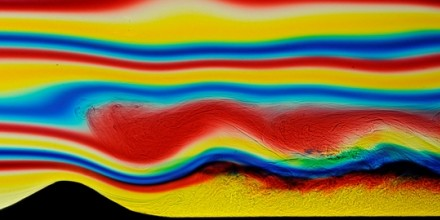
\includegraphics[height=\paperheight]{gfd}
};
\end{tikzpicture}
\begin{center}	
	\Large
	\vspace{0.5cm}
	\textcolor{white}{\textbf{``Full screen figure"}\\
	\vspace{0.5cm}
    With text
    }
\end{center}
\end{frame}


%%%%%%%%%%%%%%%%%%%%%%%%%%%%%%%%%%%%%%%%%%%%%
%%%%%%%%%%%%%% FRAME: %%%%%%%%%%%%%%%%%%%%%%%%%
%%%%%%%%%%%%%%%%%%%%%%%%%%%%%%%%%%%%%%%%%%%%%
\subsection{Subsection}
\subsubsection{Subsubsection}

\begin{frame}{Video}
\begin{figure}[ht]
	\vspace{-1cm}
	\hspace*{-2.0cm}
	\includemovie[
	poster,autostart,loop,
	text={\small(Loading video)}
	]{14cm}{7.5cm}{./videos/global_ocean.mp4}
\end{figure}
%\huge Animation with eddies and jets interacting
\end{frame}

%%%%%%%%%%%%%%%%%%%%%%%%%%%%%%%%%%%%%%%%%%%%%
%%%%%%%%%%%%%% FRAME: %%%%%%%%%%%%%%%%%%%%%%%%%
%%%%%%%%%%%%%%%%%%%%%%%%%%%%%%%%%%%%%%%%%%%%%

\begin{frame}{Navier-Stokes Equation}
\begin{equation*}
\begin{aligned}
\underbrace{\rho\frac{D\vec{u}}{Dt}}_{Total\ derivative} = & \underbrace{-\nabla p}_{Pressure\ gradient} + 
& \underbrace{\rho \vec{g}}_{Body\ force\ term} \\
& \underbrace{\mu\nabla^2\vec{u}}_{Diffusion\ term}\\
\label{eq:eke_de}
\end{aligned}
\end{equation*}
\end{frame}

\section{Section}

\end{document}
